%% Bulletin of Mathematical Biology submission (Springer Nature LaTeX template sn-jnl, v3.1 Dec 2024)
%% lineno: continuous line numbers for review
\documentclass[pdflatex,sn-mathphys-ay,lineno]{sn-jnl}% BMB: author-year citations

\usepackage[T1]{fontenc}
\usepackage{lmodern}

\usepackage{graphicx}
\usepackage{multirow}
\usepackage{amsmath,amssymb,amsfonts}
\usepackage{xcolor}
\usepackage{textcomp}
\usepackage{booktabs}
\usepackage{array}
\usepackage{tikz}
\usetikzlibrary{arrows.meta,positioning,shapes.geometric}
\usepackage{algorithm}
\usepackage{algorithmic}
\usepackage{capt-of}
\usepackage{enumitem}

\newcommand{\btheta}{\boldsymbol{\theta}}
\newcommand{\bphi}{\boldsymbol{\phi}}
\newcommand{\bpsi}{\boldsymbol{\psi}}
\newcommand{\yobs}{\mathbf{y}_{\mathrm{obs}}}
\newcommand{\Real}{\mathbb{R}}
% Values awaiting the final runs; red in the PDF so that none is left unnoticed
\newcommand{\TBD}[1]{\textcolor{red}{\textbf{[#1]}}}

\raggedbottom

\begin{document}

\title[Bayesian inference of oral biofilm interactions]{Inferring effective interactions in a multispecies oral biofilm model: Bayesian calibration and a testable prediction}

\author*[1,2,3,4]{\fnm{Keisuke} \sur{Nishioka}}\email{keisuke.nishioka@stud.uni-hannover.de}
\author[1]{\fnm{Felix} \sur{Klempt}}
\author[1]{\fnm{Hendrik} \sur{Geisler}}
\author[2,3]{\fnm{Rumjhum} \sur{Mukherjee}}
\author[2,3]{\fnm{Nils} \sur{Heine}}
\author[2,3]{\fnm{Katharina} \sur{Doll-Nikutta}}
\author[2,3]{\fnm{Meike} \sur{Stiesch}}
\author[2,3]{\fnm{Szymon P.} \sur{Szafra\'{n}ski}}
\author[1]{\fnm{Meisam} \sur{Soleimani}}
\author[1]{\fnm{Philipp} \sur{Junker}}

\affil*[1]{\orgdiv{Institute of Continuum Mechanics}, \orgname{Leibniz Universit\"at Hannover}, \orgaddress{\street{An der Universit\"at 1}, \city{Garbsen}, \postcode{30823}, \country{Germany}}}
\affil[2]{\orgdiv{Department of Prosthetic Dentistry and Biomedical Materials Science}, \orgname{Hannover Medical School}, \orgaddress{\city{Hannover}, \country{Germany}}}
\affil[3]{\orgname{Lower Saxony Centre for Biomedical Engineering, Implant Research and Development (NIFE)}, \orgaddress{\city{Hannover}, \country{Germany}}}
\affil[4]{\orgdiv{School of Science for Open and Environmental Systems, Graduate School of Science and Technology}, \orgname{Keio University}, \orgaddress{\city{Yokohama}, \country{Japan}}}

\abstract{We present a GPU-accelerated Bayesian framework for inferring the interaction parameters of a five-species oral biofilm model derived from the extended Hamilton principle.
The symmetric $5\times5$ interaction matrix is parametrised by its 15 independent entries.
Inference proceeds in stages: the likelihood first contains the species composition only, and the community viability is then added as a further channel.
The forward model is compiled with JAX and evaluated for all particles in parallel on a GPU, giving a $\sim$150$\times$ speed-up over the CPU baseline.
No interaction parameter is fixed to zero a priori, and every inference stage is checked with independent seeds against explicit convergence criteria.
Applied to in-vitro time-course data of Heine et al.\ under four combinations of community state (commensal vs.\ dysbiotic) and cultivation (static vs.\ dynamic, the latter in a HOBIC flow reactor), the inferred effective parameters reproduce the observed trajectories, including the late \textit{P.~gingivalis} (Pg) increase under dysbiotic dynamic cultivation (RMSE \TBD{0.05--0.12}).
The \textit{F.~nucleatum} (Fn)--Pg coefficient is positive in that condition (90\% interval \TBD{[+0.8, +5.2]}), positive under dysbiotic static cultivation only within the dominant of two posterior modes, and indistinguishable from zero in both commensal conditions.
The inferred model reproduces the measured pH under dynamic cultivation, which is not used in the inference ($R^2=\TBD{0.78}$ through a fixed regression on the species fractions). Posterior predictive simulations without Fn suppress the late Pg increase with probability \TBD{0.87--0.90}, yielding a directly testable prediction.}

\keywords{Bayesian inference, transitional Markov chain Monte Carlo, oral biofilm, multi-species interaction, parameter identification, peri-implantitis}

\maketitle


%==============================================================================
\section{Introduction}
\label{sec:intro}
%==============================================================================

Multi-species biofilms that form on dental implant surfaces are a principal etiological factor in peri-implantitis~\citep{Kolenbrander2010OralMultispecies, Marsh2003Dental}. Recent \textit{in vivo} characterisations indicate that these microbial communities are highly complex, individualized, and dynamically structured over time~\citep{dieckow2024structure, cui2025microbial}.
In a controlled in vitro study, \citet{heine2025influence} investigated the temporal dynamics of five representative oral taxa, \textit{Streptococcus oralis} (\textit{So}), \textit{Actinomyces naeslundii} (\textit{An}), \textit{Veillonella} spp.\ (\textit{Vei}; \textit{V.~dispar} in commensal, \textit{V.~parvula} in dysbiotic conditions), \textit{Fusobacterium nucleatum} (\textit{Fn}), and \textit{Porphyromonas gingivalis} (\textit{Pg}), across four experimental conditions defined by community state (commensal vs. dysbiotic) and cultivation mode (static vs. HOBIC reactor).
Importantly, the two community states incorporated distinct \textit{Porphyromonas gingivalis} strains: the commensal consortium included the avirulent strain \textit{Pg} DSM\,20709, whereas the dysbiotic consortium employed the virulent strain \textit{Pg} W83, which harbors a full complement of gingipain and fimbrial virulence determinants~\citep{heine2025influence}.
Building on the extended Hamilton principle~\citep{JunkerBalzani2021ExtendedHamilton}, \citet{Klempt2025ContinuumBiofilm} formulated a continuum model in which a symmetric interaction matrix~$\mathbf{A}$ governs species growth, with an optional decay vector~$\mathbf{b}$ for antibiotic effects.
\citet{Fritsch2025BayesianMicrofilms} subsequently introduced Bayesian updating with surrogate models for biofilm parameter estimation under hybrid uncertainties.

Despite these advances, estimating the 15-dimensional parameter vector (15 interaction parameters) from limited time-course data remains challenging.
Two principal difficulties arise: (i) poor identifiability when data are sparse relative to the parameter dimension---with $N_t=5$ usable time points (Day~1 is consumed as initial condition) and 5 species, one has at most 25 observations for 15 unknowns---and (ii) multimodal posterior landscapes caused by the coupled $\phi_i$--$\psi_i$ dynamics, which render standard MCMC methods inefficient~\citep{RobertCasella2004MonteCarlo}.

In this work we address these challenges through three complementary strategies.
First, we introduce the data in two phases: the interaction matrix is first inferred from the species composition alone, and the viability (and, for HOBIC cultivation, pH) measurements are added only once the composition-based posterior is available.
Second, we compile the forward model in JAX~\citep{jax2018github} and evaluate the entire particle ensemble on GPU via batched \texttt{vmap}, achieving a $\sim$150$\times$ speedup over the CPU baseline.
Third, we infer the posterior with TMCMC~\citep{ChingChen2007TMCMC, Betz2016TMCMC} in stages with progressively narrowed prior boxes and verify every stage with independent seeds and explicit convergence criteria (Section~\ref{sec:convergence}).
The framework is applied to all four experimental conditions of Heine et al.; it reproduces commensal homeostasis as well as the late pathogen increase of dysbiotic biofilms under HOBIC flow, and it yields a prediction that can be tested by a leave-one-species-out experiment.

%==============================================================================
\section{Mathematical model}
\label{sec:model}
%==============================================================================

\subsection{State variables and kinematics}

Following \citet{Klempt2025ContinuumBiofilm, Klempt2024ContinuumGrowth}, the biofilm is described at a material point by two sets of internal variables: the volume fraction $\phi_i \in [0,1]$ occupied by species~$i$ ($i=1,\dots,n$; here $n=5$), and the viability fraction $\psi_i \in [0,1]$ representing the proportion of living cells within species~$i$.
The living volume fraction is then
\begin{equation}
\bar{\phi}_i := \phi_i\,\psi_i,
\qquad i=1,\dots,n.
\label{eq:living}
\end{equation}
An additional void fraction~$\phi_0$ closes the system via the holonomic constraint
\begin{equation}
\sum_{l=0}^{n}\phi_l(t) - 1 = 0 \quad\forall\,t.
\label{eq:constraint}
\end{equation}

% \subsection{Variational formulation}

% The evolution equations are derived from the extended Hamilton principle~\citep{JunkerBalzani2021ExtendedHamilton, JunkerBodeHackl2025Holistic}
% \begin{equation}
% \mathcal{H} = \int_\tau \bigl(\mathcal{G} + \mathcal{C} + \mathcal{D}\bigr)\,\mathrm{d}t \to \mathrm{stat}_{\boldsymbol{\xi},\gamma}\,,
% \label{eq:hamilton}
% \end{equation}
% where $\boldsymbol{\xi}=(\boldsymbol{\phi},\boldsymbol{\psi})^T$ collects the volume fractions and viability fractions, $\gamma$ is a Lagrange multiplier enforcing the volume constraint, $\mathcal{G}$ is the Helmholtz free energy, $\mathcal{C}$ the constraint functional, and $\mathcal{D}$ the dissipation.
% The free energy density encodes nutrient-driven growth and antibiotic-induced killing:
% \begin{equation}
% \Psi = -\tfrac{1}{2}\,c^*\,\bar{\bphi}^T \mathbf{A}\,\bar{\bphi}
%       + \tfrac{1}{2}\,\alpha^*\,\bpsi^T \mathbf{B}\,\bpsi,
% \label{eq:psi}
% \end{equation}
% where $c^*$ is the nutrient concentration, $\alpha^*$ the antibiotic concentration, $\mathbf{A}\in\Real^{n\times n}$ the symmetric growth coefficient matrix, and $\mathbf{B}=\mathrm{diag}(b_1,\dots,b_n)$ the antibiotic sensitivity matrix.
% The volume constraint~\eqref{eq:constraint} enters through a Lagrange multiplier~$\gamma$:
% \begin{equation}
% C = \gamma\Bigl(\sum_{l=0}^{n}\phi_l - 1\Bigr).
% \label{eq:cfunc}
% \end{equation}
% The dissipation function is modeled as from the rate-dependent potential~\citep{Klempt2025ContinuumBiofilm}
% \begin{equation}
% \mathbf{\Delta} = \tfrac{1}{2}\,\dot{\bar{\bphi}}^T\boldsymbol{\eta}\,\dot{\bar{\bphi}}
%           + \tfrac{1}{2}\,\dot{\bphi}^T\boldsymbol{\eta}\,\dot{\bphi},
% \label{eq:dissipation}
% \end{equation}
% with the diagonal viscosity matrix $\boldsymbol{\eta}=\mathrm{diag}(\eta_1,\dots,\eta_n)$.
% The first term couples $\dot\phi_i$ and $\dot\psi_i$ through $\dot{\bar\phi}_i = \dot\phi_i\psi_i + \phi_i\dot\psi_i$, giving rise to non-linear dissipative interactions; the second term regularises the system to full rank.
% Following \citet{Klempt2025ContinuumBiofilm}, the viscosity parameters are set to $\eta_i=1$ for all species, rendering them dimensionless scaling factors; the physical time scale is absorbed into the time-step size $\Delta t$.

\subsection{Variational formulation}
The evolution equations are derived from the principle of the minimum of the dissipation potential \citep{junker2014principle, hackl1997generalized}, which is a local form of
\begin{equation}
    \dot{\Psi} + \Delta + C \rightarrow \mathrm{stat}_{(\dot{\boldsymbol{\xi}}, \, \gamma)},
    \label{eq:variational_local}
\end{equation}
where $\boldsymbol{\xi} = (\boldsymbol{\phi}, \boldsymbol{\psi})^T$ collects the volume fractions and viability fractions, $\gamma$ is a Lagrange multiplier enforcing the volume constraint, $C$ is the constraint function, and $\Delta$ the dissipation function. The free energy density encodes nutrient-driven growth and antibiotic-induced killing:
\begin{equation}
\Psi = -\tfrac{1}{2}\,c^*\,\bar{\bphi}^T \mathbf{A}\,\bar{\bphi}
      + \tfrac{1}{2}\,\alpha^*\,\bpsi^T \mathbf{B}\,\bpsi,
\label{eq:psi}
\end{equation}
where $c^*$ is the nutrient concentration, $\alpha^*$ the antibiotic concentration, $\mathbf{A}\in\Real^{n\times n}$ the symmetric growth coefficient matrix, and $\mathbf{B}=\mathrm{diag}(b_1,\dots,b_n)$ the antibiotic sensitivity matrix.

The dissipation function is derived from the rate-dependent potential~\citep{Klempt2025ContinuumBiofilm}:
\begin{equation}
\Delta = \tfrac{1}{2}\,\dot{\bar{\bphi}}^T\boldsymbol{\eta}\,\dot{\bar{\bphi}}
          + \tfrac{1}{2}\,\dot{\bphi}^T\boldsymbol{\eta}\,\dot{\bphi},
\label{eq:dissipation}
\end{equation}
with the diagonal viscosity matrix $\boldsymbol{\eta}=\mathrm{diag}(\eta_1,\dots,\eta_n)$. The first term couples $\dot\phi_i$ and $\dot\psi_i$ through $\dot{\bar\phi}_i = \dot\phi_i\psi_i + \phi_i\dot\psi_i$, giving rise to non-linear dissipative interactions; the second term regularises the system to full rank. Following \citet{Klempt2025ContinuumBiofilm}, the viscosity parameters are set to $\eta_i=1$ for all species, rendering them dimensionless scaling factors; the physical time scale is absorbed into the time-step size $\Delta t$.

The volume constraint~\eqref{eq:constraint} enters through a Lagrange multiplier~$\gamma$:
\begin{equation}
C = \gamma\Bigl(\sum_{l=0}^{n}\phi_l - 1\Bigr).
\label{eq:cfunc}
\end{equation}


\subsection{Governing equations}

% Evaluating $\delta\mathcal{H}=0$ with respect to variations $\delta\phi_i$, $\delta\psi_i$, and $\delta\gamma$ yields the coupled evolution equations~\citep{Klempt2025ContinuumBiofilm}:

Evaluating the stationarity conditions yields the coupled evolution equations~\citep{Klempt2025ContinuumBiofilm}:

\medskip\noindent
\textit{Volume fraction} ($i=1,\dots,n$):
\begin{equation}
0 = -c^*\,\psi_i\,\bigl(\mathbf{A}\bar{\bphi}\bigr)_i
    + \eta_i\bigl(\dot\phi_i\,\psi_i^2 + \bar\phi_i\,\dot\psi_i + \dot\phi_i\bigr)
    + \gamma,
\label{eq:phi}
\end{equation}

\noindent\textit{Viability fraction} ($i=1,\dots,n$):
\begin{equation}
0 = -c^*\,\phi_i\,\bigl(\mathbf{A}\bar{\bphi}\bigr)_i
    + \alpha^*\,b_i\,\psi_i
    + \eta_i\bigl(\dot\psi_i\,\phi_i^2 + \bar\phi_i\,\dot\phi_i\bigr)
    + \gamma,
\label{eq:psi_evol}
\end{equation}

\noindent\textit{Void fraction}:
\begin{equation}
0 = \gamma + \dot\phi_0,
\label{eq:phi0}
\end{equation}

\noindent\textit{Volume constraint}:
\begin{equation}
0 = \sum_{l=0}^{n}\phi_l - 1,
\label{eq:constraint_eq}
\end{equation}
In the numerical implementation, a logarithmic barrier penalty $\Psi_{\mathrm{bar}}$ with $K_p=\eta_i\times10^{-4}$ is added to enforce the box constraints $\phi_i,\psi_i\in[0,1]$~\citep{Klempt2025ContinuumBiofilm}; its contribution is omitted from Eqs.~\eqref{eq:phi}--\eqref{eq:phi0} for clarity.
The system~\eqref{eq:phi}--\eqref{eq:constraint_eq} constitutes $2n+2$ coupled non-linear equations for the unknowns $(\phi_1,\dots,\phi_n,\phi_0,\psi_1,\dots,\psi_n,\gamma)$, solved at each time step via Newton's method with an implicit Euler discretisation ($\Delta t = 10^{-4}$, $N_{\mathrm{step}}=2{,}500$ steps, $t_{\max}=0.25$ corresponding to the 21-day experimental window).

The variational derivation automatically ensures symmetry $A_{ij}=A_{ji}$ and thermodynamic consistency~\citep{JunkerBalzani2021ExtendedHamilton}.
Since $c^*$ enters the evolution equations only through the product $c^*A_{ij}$, its absolute value is non-identifiable; we fix $c^*=25$ so that the inferred $A_{ij}$ remain $\mathcal{O}(1)$.
The Heine et al.\ experiments do not involve antibiotic agents, so we set $\alpha^*=0$, which eliminates the decay term $\alpha^*b_i\psi_i$ from Eq.~\eqref{eq:psi_evol}; the antibiotic sensitivity matrix~$\mathbf{B}$ is therefore inactive and excluded from estimation.
The symmetric interaction matrix~$\mathbf{A}$ has 15 independent entries (Section~\ref{sec:model_matrix}); these form the 15-dimensional parameter vector~$\btheta$.
Removing a species from the consortium is represented by switching it off (its volume fraction is held at zero), not by a zero initial value: in this formulation a species with a vanishing initial fraction can regrow from numerical floor values.

\subsection{Symmetric interaction matrix}
\label{sec:model_matrix}

The symmetry $A_{ij}=A_{ji}$ arises automatically from the quadratic form of the free energy~\eqref{eq:psi}, reducing the off-diagonal degrees of freedom from 20 to~10.
Together with the 5 diagonal entries, the symmetric matrix has 15 independent entries.
These are distinct from the antibiotic sensitivity parameters~$b_i$ in Eq.~\eqref{eq:psi_evol}, which vanish when $\alpha^*=0$.
The resulting 15-dimensional parameter vector is
\begin{equation}
\btheta = (\theta_0,\dots,\theta_{14})^T \in \Real^{15},
\label{eq:theta}
\end{equation}
organised into five biologically motivated blocks:
\begin{equation}
\btheta =
\underbrace{(a_{11},a_{12},a_{22})}_{\text{So--An}}
\oplus
\underbrace{(a_{33},a_{34},a_{44})}_{\text{Vei--Fn}}
\oplus
\underbrace{(a_{13},a_{14},a_{23},a_{24})}_{\text{cross}}
\oplus
\underbrace{(a_{15},a_{25},a_{35},a_{45})}_{\text{Pg cross}}
\oplus
\underbrace{(a_{55})}_{\text{Pg}}.
\label{eq:blocks}
\end{equation}

\subsection{Biological interaction network}

Figure~\ref{fig:network} summarises previously reported or biologically supported interactions among the five taxa, compiled from \citet{heine2025influence} and the literature; it is used only to interpret the inferred parameters, not as a constraint.
The listed pairs rest on different kinds of evidence (co-aggregation, metabolic cross-feeding, pH modification, peptide utilisation), which Table~\ref{tab:active} states for each pair.
Because $\mathbf{A}$ is symmetric by construction, an inferred coefficient $a_{ij}$ describes an undirected effective interaction between species $i$ and $j$; the arrow in Figure~\ref{fig:network} represents a metabolite flow reported in the literature, not a direction recovered by the model.
All 15 entries of $\mathbf{A}$ are estimated (i.e., no $\theta_k\equiv0$), so that no reported interaction is imposed and no unreported one is excluded.

\begin{figure}[htbp]
\centering
\begin{minipage}[t]{0.32\textwidth}
\vspace{0pt}
\centering
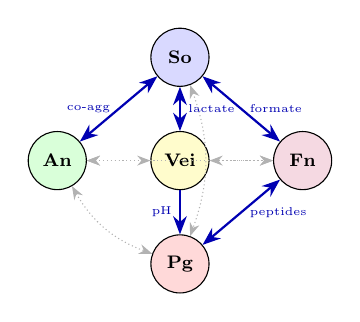
\begin{tikzpicture}[scale=0.82, every node/.style={transform shape},
    species/.style={circle, draw, minimum size=0.9cm, font=\footnotesize\bfseries},
    edge/.style={<->, thick, >=Stealth},
    uniedge/.style={->, thick, blue!70!black, >=Stealth},
    weakedge/.style={<->, thin, gray!60, >=Stealth, densely dotted}
]
    \node[species, fill=blue!15] (so) at (0, 2.2) {So};
    \node[species, fill=green!15] (an) at (-1.9, 0.6) {An};
    \node[species, fill=yellow!20] (vei) at (0, 0.6) {Vei};
    \node[species, fill=purple!15] (fn) at (1.9, 0.6) {Fn};
    \node[species, fill=red!15] (pg) at (0, -1.0) {Pg};
    \draw[edge, blue!70!black] (so) -- (an) node[midway, left, font=\tiny] {co-agg};
    \draw[edge, blue!70!black] (so) -- (vei) node[midway, right, font=\tiny] {lactate};
    \draw[edge, blue!70!black] (so) -- (fn) node[midway, right, font=\tiny] {formate};
    \draw[uniedge] (vei) -- (pg) node[midway, left, font=\tiny] {pH};
    \draw[edge, blue!70!black] (fn) -- (pg) node[midway, right, font=\tiny] {peptides};
    \draw[weakedge] (an) -- (vei);
    \draw[weakedge] (an) -- (fn);
    \draw[weakedge] (vei) -- (fn);
    \draw[weakedge] (so) to[bend left=20] (pg);
    \draw[weakedge] (an) to[bend right=20] (pg);
\end{tikzpicture}
\end{minipage}%
\hfill
\begin{minipage}[t]{0.65\textwidth}
\vspace{0pt}
\small
\begin{tabular}{@{}lll@{}}
\toprule
\textbf{Pair} & \textbf{Mechanism} & \textbf{Reported flow}\\
\midrule
So--An & Co-aggregation & mutual\\
So--Vei & Lactate exchange & So to Vei\\
So--Fn & Formate symbiosis & mutual\\
Vei--Pg & pH elevation & Vei to Pg\\
Fn--Pg & Peptide supply & mutual\\
\bottomrule
\end{tabular}
\captionof{table}{Previously reported or biologically supported interactions~\citep{heine2025influence} used to interpret the inferred coefficients. The model coefficients $a_{ij}$ are symmetric; the last column refers to the reported metabolite flow, not to the model. All 15 parameters are estimated; none is fixed a priori.}
\label{tab:active}
\end{minipage}
\caption{Species interaction network~\citep{heine2025influence}. Solid: previously reported or biologically supported interactions considered in the interpretation of the model. Dotted grey: no reported pathway. All pairs are estimated with the same prior.}
\label{fig:network}
\end{figure}

The block symbols $a_{ij}$ follow the 1-based notation of \citet{Klempt2025ContinuumBiofilm}; the matrix entries $A_{ij}$ use 0-based indexing consistent with Eqs.~\eqref{eq:phi}--\eqref{eq:psi_evol}.

%==============================================================================
\section{Bayesian inference framework}
\label{sec:bayes}
%==============================================================================

\subsection{Posterior distribution}

Given observed time-course data $\yobs = \{y_{\mathrm{obs},i}(t_k)\}$, we seek the posterior
\begin{equation}
p(\btheta\mid\yobs)
= \frac{p(\yobs\mid\btheta)\,p(\btheta)}{p(\yobs)},
\label{eq:bayes}
\end{equation}
where $p(\yobs\mid\btheta)$ is the likelihood, $p(\btheta)$ the prior, and $p(\yobs)$ the model evidence.

\subsection{Likelihood}
\label{sec:likelihood}

The observations are the species fractions at Days~3, 6, 10, 15 and 21, normalised to unit sum at each time point; Day~1 serves as the initial condition and is excluded from the likelihood.
The model predicts volume fractions $\phi_i(t)$ together with a void fraction that is not observed; predictions are therefore renormalised to species fractions, $\hat{y}_i(t_k;\btheta)=\phi_i(t_k)\big/\sum_{j}\phi_j(t_k)$, before comparison.
Model time is mapped linearly to experimental days.
The initial condition is the normalised Day-1 observation, with a lower bound of $10^{-3}$ on each fraction.

For the species composition we use a weighted Gaussian log-likelihood
\begin{equation}
\ln p(\yobs\mid\btheta)
= -\frac12\sum_{k=1}^{N_t}\sum_{i=1}^{5} w_{ik}\,
\frac{\bigl(y_{\mathrm{obs},i}(t_k)-\hat{y}_i(t_k;\btheta)\bigr)^2}{\sigma_i^2} + \text{const},
\label{eq:likelihood}
\end{equation}
where $\sigma_{i}$ is a species-specific observation noise derived from the replicate standard deviation of the normalised species fractions~\citep{heine2025influence} ($N=8$ biological replicates per condition), averaged over time points.
The weights $w_{ik}$ are listed in Table~\ref{tab:weights}: Pg is up-weighted ($\lambda_{\mathrm{Pg}}=5$) because it is a low-abundance species whose late increase is the main dynamic feature of the dysbiotic data; the last two time points are up-weighted ($\lambda_{\mathrm{late}}=3$); and species whose mean fraction is below 5\% are down-weighted ($\lambda_{\mathrm{rare}}=0.1$).

In Phase~2 (Section~\ref{sec:prior}) a further Gaussian channel is added with the weight of Table~\ref{tab:weights}.
The \emph{viability channel} compares the predicted community viability $\sum_i\phi_i\psi_i/\sum_i\phi_i$ with the measured fraction of membrane-intact cells~\citep{heine2025influence}, with $\sigma_\psi$ the mean reported measurement error.
The measured pH time series of the HOBIC conditions~\citep{heine2025influence} is not used in the likelihood; it is kept for the check in Section~\ref{sec:validation}.
Treating the compositional data with independent Gaussian errors ignores the unit-sum constraint; \TBD{effect assessed in a sensitivity analysis -- to be agreed with M.S.}.

\begin{table}[htbp]\centering\small
\begin{tabular}{@{}lll@{}}\toprule
Weight & Value & Applies to\\\midrule
$\lambda_{\mathrm{Pg}}$ & 5 & Pg, all time points\\
$\lambda_{\mathrm{late}}$ & 3 & Days 15 and 21, all species\\
$\lambda_{\mathrm{rare}}$ & 0.1 & species with mean fraction $<5\%$\\
$\lambda_{\psi}$ & 3.0 (DH), 2.0 (DS), 1.5 (CS, CH) & viability channel, Phase~2\\\bottomrule
\end{tabular}
\caption{Likelihood weights.}
\label{tab:weights}
\end{table}

\subsection{Prior and inference stages}
\label{sec:prior}

The prior is a product of independent uniform distributions:
\begin{equation}
p(\btheta) = \prod_{k=0}^{14} \frac{1}{u_k-l_k}\,\mathbf{1}_{[l_k,u_k]}(\theta_k),
\label{eq:prior}
\end{equation}
on condition-specific boxes $[l_k,u_k]$ (Supplementary Table~S1).
All 15 entries of $\mathbf{A}$ are estimated in every condition; no entry is fixed a priori.
The decay vector $\mathbf{b}$ does not enter the model without antibiotic treatment ($\alpha^*=0$) and is not estimated.
The initial box was set empirically to contain earlier posterior estimates; it encodes no sign constraint. Where posterior mass accumulated at a bound of this box (more than 20\% of the mass in the outer 5\% of the range) at any stage, the box was widened for that entry and the stage was repeated: to $[-15,20]$ for $a_{33}$, $a_{34}$ and $a_{45}$ for Dysbiotic Static, for $a_{23}$, $a_{24}$, $a_{33}$, $a_{34}$ and $a_{35}$ for Dysbiotic HOBIC, and for $a_{33}$ for Commensal Static, where $a_{11}$ was also widened to $[-5,2]$ and the upper bound of $a_{13}$ raised to $20$; the lower bounds of $a_{12}$, $a_{14}$ and $a_{15}$ were lowered to $-5$ for Commensal HOBIC (for this condition the posterior of $a_{13}$ in stages (iii)--(iv) lies close to its lower bound $-1$, with a 5\% quantile of \TBD{$-0.93$}, below the widening threshold); the lower bounds of $a_{15}$, $a_{23}$ and $a_{55}$ were lowered to $-5$ for Dysbiotic Static from stage~(iii) on; in addition, $a_{11}$ and $a_{14}$ were widened to $[-5,5]$ and $[-3,3]$ and the upper bound of $a_{45}$ was raised from $6$ to $20$ for Dysbiotic HOBIC from stage~(iii) on \TBD{confirm with the final runs}.

Inference proceeds in four stages that share the same data:
(i)~composition likelihood on the initial box;
(ii)~composition likelihood, box narrowed to the stage-(i) posterior mean $\pm4$ posterior standard deviations (SDs);
(iii)~composition and viability likelihood on the initial box, starting from the stage-(ii) particles (the box is not narrowed, because the likelihood changes between (ii) and (iii) and a box derived from the stage-(ii) posterior truncated the stage-(iii) posterior);
(iv)~as (iii), with the box narrowed to the stage-(iii) posterior mean $\pm4$ SDs and $N_p=5{,}000$ particles.
We refer to stages (i)--(ii) as Phase~1 and to stages (iii)--(iv) as Phase~2.
Narrowing is clipped to the initial box; a $\pm4$\,SD box removes less than 0.01\% of a Gaussian marginal, so it shortens the tempering without truncating the posterior (a $\pm2$\,SD box would remove about 5\% of each well-determined marginal; results with $\pm2$\,SD are given in Supplementary Section~S4). Stages (ii)--(iv) start from a mixture of particles drawn around the previous stage's MAP and draws from the stage prior; because the initial population is then not a sample from the prior, their log-evidence estimates are not used \TBD{drop the $\ln\hat{Z}$ columns of Table~\ref{tab:rmse} or report stage (i) only}.
Because the data are reused across stages, we report alongside the final posterior the stage-(i) posterior, which involves no data-dependent narrowing, and an inference on a much wider box ($[-15,20]$ for all entries) with and without an additional $\mathcal{N}(0,6^2)$ prior (Section~\ref{sec:sensitivity}).
We monitor the fraction of posterior mass within 5\% of each bound at every stage.

%==============================================================================
\section{TMCMC inference}
\label{sec:tmcmc}
%==============================================================================

\subsection{Tempered likelihood sequence}

TMCMC~\citep{ChingChen2007TMCMC, DelMoral2006SMC, Chopin2002SMC} constructs a sequence of intermediate distributions
\begin{equation}
p_m(\btheta) \propto p(\yobs\mid\btheta)^{\beta_m}\,p(\btheta),
\qquad
0=\beta_0<\beta_1<\cdots<\beta_M=1,
\label{eq:tempered}
\end{equation}
interpolating from the prior ($\beta_0=0$) to the full posterior ($\beta_M=1$).
The tempering parameter $\beta_{m+1}$ is determined adaptively so that the coefficient of variation of the importance weights
\begin{equation}
w_j^{(m)} = p(\yobs\mid\btheta_j^{(m)})^{\beta_{m+1}-\beta_m},
\qquad j=1,\dots,N,
\label{eq:weights}
\end{equation}
satisfies $\mathrm{CoV}[\{w_j^{(m)}\}]=\delta_{\mathrm{target}}$, solved by bisection on $(\beta_m,1]$~\citep{Betz2016TMCMC}.

\subsection{Resampling and mutation}

At each stage~$m$:
\begin{enumerate}[nosep,leftmargin=*]
\item \textbf{Resample} $N$ particles from $\{\btheta_j^{(m)}\}$ with probabilities $\propto w_j^{(m)}$.
\item \textbf{Estimate} the weighted covariance
\begin{equation}
\boldsymbol{\Sigma}^{(m)}
= \sum_{j=1}^{N}\bar{w}_j^{(m)}
\bigl(\btheta_j^{(m)}-\bar{\btheta}^{(m)}\bigr)
\bigl(\btheta_j^{(m)}-\bar{\btheta}^{(m)}\bigr)^T.
\label{eq:cov}
\end{equation}
\item \textbf{Mutate} each particle via Metropolis--Hastings with proposal $q(\btheta^*\mid\btheta_j)=\mathcal{N}(\btheta_j,\gamma^2\boldsymbol{\Sigma}^{(m)})$ and acceptance probability
\begin{equation}
\alpha = \min\!\biggl(1,\;
\frac{p(\yobs\mid\btheta^*)^{\beta_{m+1}}\,p(\btheta^*)}
     {p(\yobs\mid\btheta_j)^{\beta_{m+1}}\,p(\btheta_j)}\biggr).
\label{eq:accept}
\end{equation}
Proposals outside the prior box are rejected without evaluating the likelihood.
\end{enumerate}
Random-walk proposals alternate with differential-evolution proposals~\citep{terBraak2006DEMC}, $\btheta^*=\btheta_j+\gamma_{\mathrm{DE}}(\btheta_a-\btheta_b)+\boldsymbol{\epsilon}$ with $\gamma_{\mathrm{DE}}=2.38/\sqrt{2d}$, which adapt to strongly correlated posteriors.
Each stage applies $K$ mutation steps to every particle (Table~\TBD{runs}).

A by-product of TMCMC is the model evidence estimate
\begin{equation}
\hat{p}(\yobs) = \prod_{m=0}^{M-1}\Bigl(\frac{1}{N}\sum_{j=1}^{N}w_j^{(m)}\Bigr),
\label{eq:evidence}
\end{equation}
which can be used for Bayesian model comparison between models fitted to the same data~\citep{KassRaftery1995BayesFactor}.
The estimate satisfies $\ln\hat{Z}\le\max_j\ln p(\yobs\mid\btheta_j)$, which we check for every run.
Because the likelihoods of different conditions involve different data, $\ln\hat{Z}$ is not compared across conditions.

\subsection{Joint estimation in 15 dimensions}

All 15 parameters are estimated jointly in every stage, made affordable by the GPU implementation of Section~\ref{sec:gpu}.
The biologically motivated blocks (Eq.~\ref{eq:blocks}) serve as interpretive groups for posterior analysis but are not estimated sequentially.

\subsection{Convergence assessment}
\label{sec:convergence}

Every stage is run with three independent seeds and accepted only if all of the following hold:
(i)~the stored log-likelihood of every particle agrees with a recomputation from the stored parameters;
(ii)~the tempering reaches $\beta=1$;
(iii)~each particle is moved on average at least twice per stage and at least five times per free parameter over the run;
(iv)~the maximum log-likelihood differs by at most 1 across seeds; and
(v)~the posterior median of every parameter differs across seeds by at most half a posterior standard deviation.
Criterion~(iii) uses accepted moves rather than the acceptance rate: with optimally scaled random-walk proposals, $5d$ accepted moves displace each coordinate by about $2.38\sqrt5\approx5$ posterior standard deviations, independently of~$d$.
Effective sample sizes after resampling are not reported, as they reflect the resampling rather than mixing.


%==============================================================================
\section{GPU-accelerated forward model}
\label{sec:gpu}
%==============================================================================

Each TMCMC run requires $\mathcal{O}(10^5)$--$\mathcal{O}(10^6)$ forward ODE solves (up to $N_p$ particles $\times$ $K$ mutation steps $\times$ $M$ tempering stages), and every stage is repeated with three seeds.
We address the resulting computational cost through GPU parallelism and a two-phase introduction of the data.

\paragraph{GPU-parallel TMCMC.}
The forward model (Eqs.~\ref{eq:phi}--\ref{eq:constraint_eq}) is implemented in JAX~\citep{jax2018github}: the implicit Euler Newton solver---including Jacobian assembly and linear solve---is compiled via \texttt{jax.jit} into a single fused XLA kernel.
All $N$ particle trajectories are evaluated simultaneously via \texttt{jax.vmap} on GPU (NVIDIA RTX\,4090 for the benchmark in Table~\ref{tab:timing}), replacing the $\lceil N/12\rceil$ serial batches required on CPU.
This yields a $\sim$200$\times$ end-to-end speedup (Table~\ref{tab:timing}).

\paragraph{Two-phase introduction of the data.}
In Phase~1 (stages (i)--(ii), Section~\ref{sec:prior}) the likelihood contains the species composition only.
The full system~\eqref{eq:phi}--\eqref{eq:constraint_eq}, including the viability fractions $\psi_i$, is integrated in both phases; since the composition is compared after renormalisation, the viability measurements carry information only through the additional channels of Phase~2.
Phase~2 (stages (iii)--(iv)) adds the viability and pH channels and starts from the Phase~1 particles on a box narrowed around the Phase~1 MAP.
Comparing Phase~1 and Phase~2 MAP estimates shows how strongly the viability and pH data move $\mathbf{A}$.

The procedure is summarised in Algorithm~\ref{alg:tmcmc}; Table~\ref{tab:timing} reports the computational gains.

\begin{algorithm}[t]
\caption{Staged GPU-accelerated TMCMC (one seed; every stage is run with three seeds and checked as in Section~\ref{sec:convergence})}
\label{alg:tmcmc}
\begin{algorithmic}[1]
\REQUIRE Composition data $\yobs$, viability data, $N_p$ particles, GPU device
\ENSURE MAP estimate $\hat{\btheta}^{\mathrm{MAP}}$, posterior samples, log-evidence $\ln\hat{Z}$
\STATE $\triangleright$ \textbf{Stage (i): composition likelihood, initial box}
\STATE Draw $\{\btheta_j\}_{j=1}^{N_p}$ from the stage prior; set $\beta_0\leftarrow 0$
\WHILE{$\beta_m < 1$}
    \STATE Find $\beta_{m+1}$ s.t.\ $\mathrm{CoV}[\{w_j\}]=\delta_{\mathrm{target}}$ via bisection
    \STATE Compute weights $w_j \leftarrow p(\yobs\mid\btheta_j)^{\beta_{m+1}-\beta_m}$
    \STATE Resample $N_p$ particles $\propto w_j$ (systematic)
    \STATE Estimate weighted covariance $\hat{\boldsymbol{\Sigma}}^{(m)}$ (Eq.~\ref{eq:cov})
    \FOR{$k = 1$ \TO $K$}
        \STATE Propose $\btheta_{j}'$ for all $j$ (random-walk or differential-evolution move)
        \STATE Evaluate all $N_p$ likelihoods in parallel via \texttt{jax.vmap} on GPU
        \STATE Accept/reject via MH (Eq.~\ref{eq:accept}); reject proposals outside the box
    \ENDFOR
\ENDWHILE
\STATE Record MAP and posterior SD per parameter
\STATE $\triangleright$ \textbf{Stage (ii): composition likelihood, box mean $\pm4$\,SD}
\STATE Repeat lines 2--13 on the narrowed box, starting from the previous particles
\STATE $\triangleright$ \textbf{Stages (iii)--(iv): add the viability channel; initial box, then mean $\pm4$\,SD}
\STATE Augment likelihood with the weighted viability channel (Table~\ref{tab:weights})
\STATE Repeat lines 2--13 for each stage
\RETURN $\hat{\btheta}^{\mathrm{MAP}}$, posterior samples, $\ln\hat{Z}$
\end{algorithmic}
\end{algorithm}

\begin{table}[htbp]
\centering\small
\begin{tabular}{@{}lrrr@{}}
\toprule
\textbf{Metric} & \textbf{CPU (12 cores)} & \textbf{GPU (RTX\,4090)} & \textbf{Speedup}\\
\midrule
\multicolumn{4}{@{}l}{\textit{Matched benchmark (DH, $N_p=500$, $K=10$, 9 stages):}}\\
\quad Per stage     & 2\,400\,s   & 14\,s    & $170\times$\\
\quad Total         & 21\,600\,s  & 147\,s   & $\mathbf{147\times}$\\
\midrule
\multicolumn{4}{@{}l}{\textit{Final stage (iv) (4 cond., $N_p=\TBD{n}$, $K=\TBD{n}$, GPU \TBD{model}):}}\\
\quad Per condition & \TBD{h}$^\dagger$ & \TBD{h} & \TBD{x}\\
\quad All 4 cond.   & \TBD{h}$^\dagger$ & \TBD{h} & \TBD{x}\\
\bottomrule
\end{tabular}
\caption{Computational cost comparison.
The matched benchmark (500 particles, identical settings) isolates the GPU speedup at about 150--170$\times$ (170$\times$ per stage, 147$\times$ in total).
The final-stage times are measured per seed \TBD{update with the final runs}.
$^\dagger$Extrapolated from the 500-particle CPU benchmark assuming linear scaling in~$N_p$.}
\label{tab:timing}
\end{table}

A large language model (Claude, Anthropic) was used to assist with code development and manuscript preparation; all code and text were reviewed and verified by the authors, who take full responsibility for the content.

%==============================================================================
\section{Results}
\label{sec:results}
%==============================================================================

The inference is performed under four experimental conditions from \citet{heine2025influence}: Commensal Static (CS), Commensal HOBIC (CH), Dysbiotic Static (DS), and Dysbiotic HOBIC (DH).
Species distribution data ($N=8$ biological replicates per condition, Days~1, 3, 6, 10, 15, 21) were normalised to unit sum at each time point; Day~1 serves as initial condition.
All 15 interaction parameters are estimated simultaneously for every condition, following the staged procedure of Section~\ref{sec:prior} and Algorithm~\ref{alg:tmcmc}.
Each stage is run with three seeds; Table~\TBD{runs} lists particles, mutation steps and number of tempering stages per condition, together with the outcome of the convergence criteria of Section~\ref{sec:convergence}.
All runs use a coefficient-of-variation target $\delta_{\mathrm{target}}=1.0$ for the adaptive $\beta$-schedule~\citep{Betz2016TMCMC} and an initial random-walk scale $\gamma^2=2.38^2/d$~\citep{RobertsRosenthal2001Optimal}.
The random-walk scale is adapted online after each random-walk step: $\gamma^2$ is multiplied by 0.5 when the acceptance rate of that step is below 10\%, by 0.8 when it is below 18\%, and by 1.3 when it exceeds 35\%; the differential-evolution scale is kept fixed.

\TBD{All numbers in this section are from the previous runs and will be replaced by the final stage-(iv) runs.}

\subsection{Quantitative fit metrics}

Table~\ref{tab:rmse} reports the composition fit at the end of Phase~1 (composition likelihood only) and Phase~2 (with the viability and pH channels).
Phase~1 fits the composition at least as well as Phase~2 in every condition, as expected since Phase~2 also has to match the viability and pH data.
In Phase~2, DS has the best composition fit (RMSE$=$0.033, $R^2_{\text{\textit{Pg}}}=0.85$), and DH reproduces the late Pg increase ($R^2_{\text{\textit{Pg}}}=0.90$).
The composition RMSE increases by at most 0.035 from Phase~1 to Phase~2.

\begin{table}[htbp]
\centering\footnotesize\setlength{\tabcolsep}{3pt}
\begin{tabular}{@{}l ccccc ccccc@{}}
\toprule
& \multicolumn{5}{c}{\textbf{Phase 1: composition only}} & \multicolumn{5}{c}{\textbf{Phase 2: with viability and pH --- final}}\\
\cmidrule(lr){2-6}\cmidrule(lr){7-11}
\textbf{Cond.} & \textbf{RMSE} & \textbf{MAE} & $\bar{\alpha}$ & $\max\ln\mathcal{L}$ & $\ln\hat{Z}$ & \textbf{RMSE} & \textbf{MAE} & $\bar{\alpha}$ & $\max\ln\mathcal{L}$ & $\ln\hat{Z}$\\
\midrule
CS  & 0.119 & 0.077 & 0.14 & $-6.3$ & $-2.6$ & 0.119 & 0.075 & 0.12 & $-21.6$ & $-3.3$\\
CH  & 0.071 & 0.053 & $\mathbf{0.17}$ & $-3.6$ & $-1.3$ & 0.104 & 0.088 & 0.07 & $-112.3$ & $-8.5$\\
DS  & $\mathbf{0.020}$ & $\mathbf{0.025}$ & 0.11 & $\mathbf{-1.2}$ & $-3.8$ & $\mathbf{0.033}$ & $\mathbf{0.024}$ & $\mathbf{0.13}$ & $-93.4$ & $-2.8$\\
DH  & 0.067 & 0.045 & 0.10 & $-6.6$ & $-9.6$ & 0.087 & 0.060 & 0.07 & $-170.4$ & $-11.9$\\
\bottomrule
\end{tabular}
\caption{Composition fit at the end of Phase~1 (stage (ii), composition likelihood only) and Phase~2 (stage (iv), with viability and pH channels).
RMSE and MAE refer to the species composition in both phases.
$\bar{\alpha}$: mean MH acceptance rate.
$\max\ln\mathcal{L}$ and $\ln\hat{Z}$ are not comparable across phases (Phase~2 includes additional channels) nor across conditions (different data); use RMSE for comparison.}
\label{tab:rmse}
\end{table}

Table~\ref{tab:r2_species} reports the per-species $R^2$ for each condition.
In commensal states (CS, CH), \textit{Fn} and \textit{Pg} fractions are near zero throughout, rendering $R^2$ undefined (total variance $\approx0$); these are marked ``$-$'' in the table.
In dysbiotic states, in Phase~1, DH achieves $R^2>0.8$ for \textit{An}, \textit{Vei}, and \textit{Pg}; in Phase~2, \textit{Vei} drops to~$0.63$ while \textit{An} ($0.86$) and \textit{Pg} ($0.90$) remain above~$0.8$.
DS achieves $R^2=0.93$ for \textit{Vei} in Phase~1 ($0.91$ in Phase~2) and $0.85$ for \textit{Pg} in both phases.
So shows negative $R^2$ in most conditions in both phases; in Phase~2 this partly reflects a trade-off between the composition and the viability and pH channels.
So also exhibits the highest replicate variability ($\sigma_{\mathrm{So}}\approx0.19$), which inflates $\mathrm{SS}_{\mathrm{tot}}$ and further depresses $R^2$.

\begin{table}[htbp]
\centering\footnotesize\setlength{\tabcolsep}{3pt}
\begin{tabular}{@{}l ccccc ccccc@{}}
\toprule
& \multicolumn{5}{c}{\textbf{Phase 1 (composition only)}} & \multicolumn{5}{c}{\textbf{Phase 2 (with viability and pH) --- final}}\\
\cmidrule(lr){2-6}\cmidrule(lr){7-11}
\textbf{Cond.} & So & An & Vei & Fn & Pg & So & An & Vei & Fn & Pg\\
\midrule
CS  & $-0.39$ & $0.80$ & $-3.2$ & $-$ & $-$ & $-0.36$ & $\mathbf{0.91}$ & $-3.7$ & $-$ & $-$\\
CH  & $0.55$  & $0.70$ & $0.59$  & $-$ & $-$ & $0.40$  & $-0.22$ & $-0.14$ & $-$ & $-$\\
DS  & $-0.87$ & $0.76$ & $\mathbf{0.93}$ & $0.54$ & $\mathbf{0.85}$ & $-0.86$ & $0.73$ & $\mathbf{0.91}$ & $0.66$ & $\mathbf{0.85}$\\
DH  & $-0.47$ & $\mathbf{0.83}$ & $\mathbf{0.83}$ & $0.60$ & $\mathbf{0.92}$ & $-0.21$ & $\mathbf{0.86}$ & $0.63$ & $0.06$ & $\mathbf{0.90}$\\
\bottomrule
\end{tabular}
\caption{Per-species $R^2$ of the composition for Phase~1 and Phase~2.
``$-$'': species fraction $<0.02$ at all time points ($\mathrm{SS}_{\mathrm{tot}}\approx0$), rendering $R^2$ ill-defined; the MAP prediction for these species is $<0.01$ with absolute error below the observation noise~$\sigma_i$.
Bold: $R^2>0.8$.
DS maintains $R^2\geq0.85$ for Vei and Pg in both phases; DH reproduces the Pg time course ($R^2=0.90$) in Phase~2.}
\label{tab:r2_species}
\end{table}

\subsection{Convergence diagnostics}

All stages of all conditions satisfy the convergence criteria of Section~\ref{sec:convergence} \TBD{table of runs: seeds, moves per parameter, spread of max log-likelihood and medians}.
The acceptance rates of \TBD{x--y}\% are below the optimum $\bar\alpha\approx23\%$ for Gaussian targets~\citep{RobertsRosenthal2001Optimal}, reflecting the non-Gaussianity and bounded support of the posterior; criterion~(iii) therefore counts accepted moves rather than relying on the acceptance rate.

\subsection{Posterior fits across conditions}

Figure~\ref{fig:fits_all} presents the posterior predictive fits for all four conditions in the order of increasing dysbiotic severity (columns left to right); each row corresponds to one species.
The solid line shows the MAP trajectory of $\varphi_i$ (total volume fraction); the dashed line shows $\bar{\varphi}_i=\varphi_i\psi_i$ (living fraction), which differs from $\varphi_i$ only where the viability $\psi_i<1$.
In CS (column~1), the model reproduces the initial rapid growth and steady state of \textit{So} and \textit{An}; pathogen species remain near zero---not due to locking, but because the posterior concentrates these entries near zero.
In CH (column~2), the So-dominated ``blue bloom'' under flow is correctly captured.
DS (column~3) achieves the best fit (RMSE\,$=$\,0.033) with clear pathogen succession under static cultivation.
In DH (column~4), the model captures the non-linear amplification of \textit{Vei} and \textit{Pg}, including the late increase of \textit{Pg}.
The credible bands widen from CS to DH, reflecting the increasing effective dimensionality.
The bottom row highlights the distinct \textit{Pg} strains: the avirulent DSM\,20709 used in commensal conditions remains near zero, whereas the virulent W83 in dysbiotic conditions increases late.
Similarly, the \textit{Veillonella} row corresponds to \textit{V.~dispar} in commensal and \textit{V.~parvula} in dysbiotic conditions~\citep{heine2025influence}.

\begin{figure}[p]
\centering
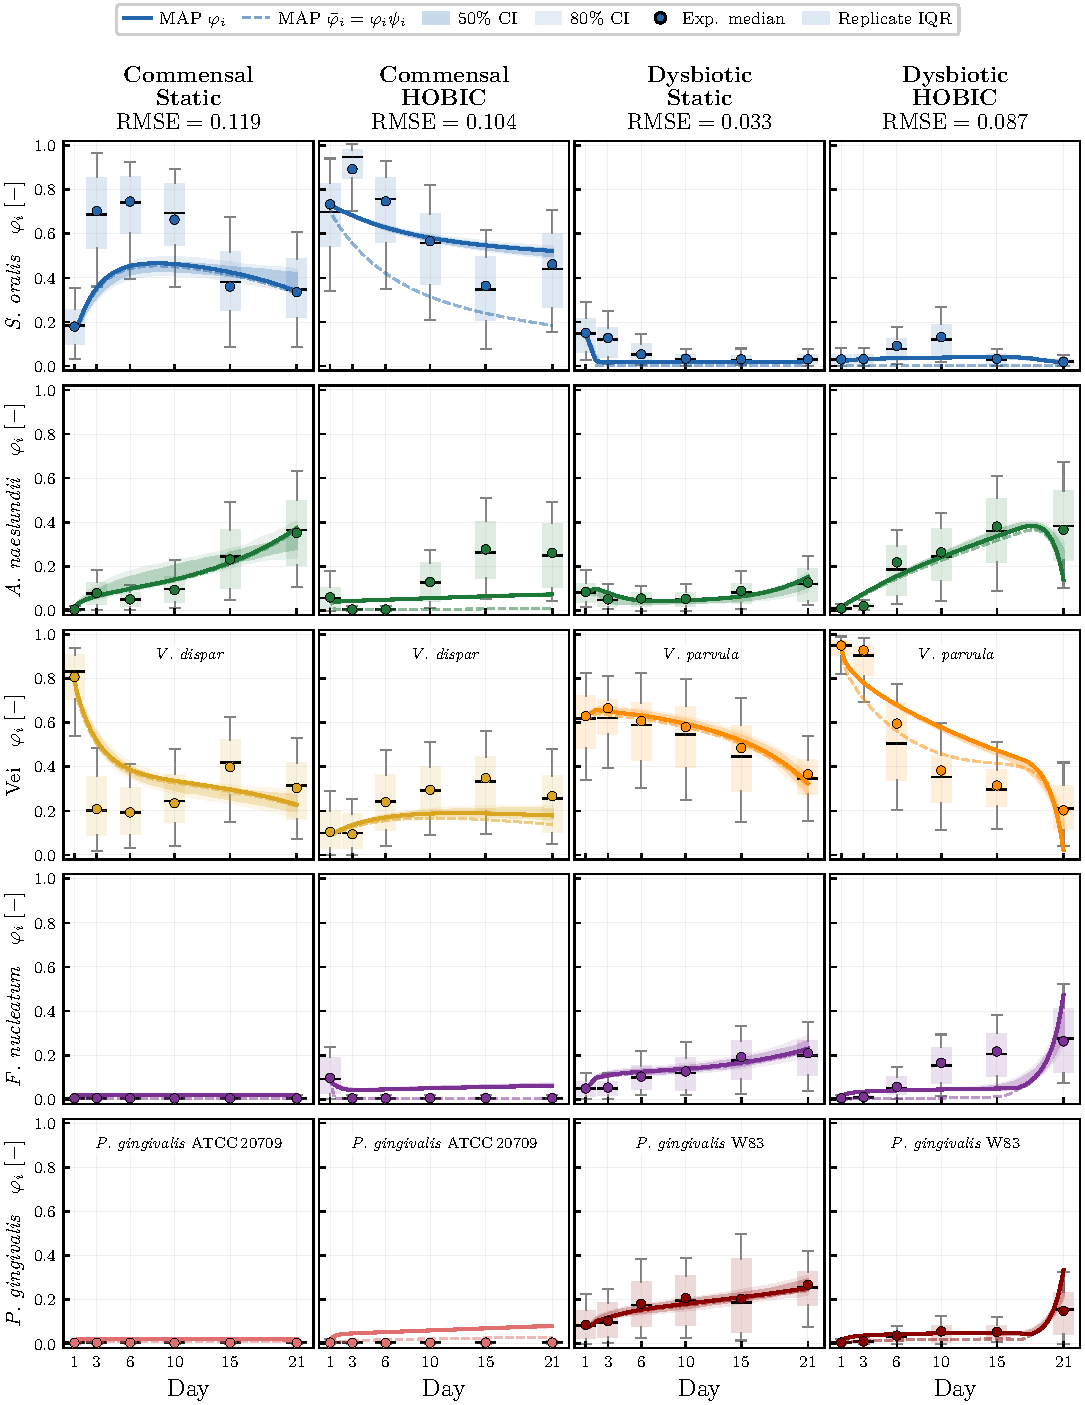
\includegraphics[width=\textwidth]{figures/paper_fig2_phi_transposed.pdf}
\caption{Posterior predictive fits of volume fraction $\varphi_i$ (Phase~2, stage (iv)). Columns: four experimental conditions (CS, CH, DS, DH); rows: five species.
Solid lines: MAP $\varphi_i$ trajectory; dashed lines: living fraction $\bar{\varphi}_i=\varphi_i\psi_i$.
Shaded bands: 50\% (dark) and 80\% (light) credible intervals from 100 posterior samples.
Circles: experimental median ($N=8$ replicates); box plots: inter-replicate variability (IQR).
Note that \textit{P.~gingivalis} employs different strains: avirulent DSM\,20709 in commensal conditions and virulent W83 in dysbiotic conditions (indicated by colour).
\textit{Veillonella} species also differ: \textit{V.~dispar} (commensal) and \textit{V.~parvula} (dysbiotic)~\citep{heine2025influence}.}
\label{fig:fits_all}
\end{figure}

\subsection{Inferred interaction matrices}

The MAP interaction matrices (Figure~\ref{fig:heatmaps}) reveal the progressive reorganisation of the interaction landscape from commensal to dysbiotic states.
In CS and CH, the dominant entries are the \textit{So}--\textit{An} and \textit{So}--\textit{Vei} blocks, reflecting the mutualistic core of early colonizers; the \textit{Fn} and \textit{Pg} rows are near zero.
In DS, pathogen-related entries appear at moderate magnitude.
In DH, the effective \textit{Vei}--\textit{Pg} and \textit{Fn}--\textit{Pg} coefficients are positive.
The MAP values of the Pg-related parameters are $\hat{a}_{55}^{\mathrm{DH}}=\TBD{3.43}$ (Pg self), $\hat{a}_{45}^{\mathrm{DH}}=\TBD{5.63}$ (Fn--Pg) and $\hat{a}_{44}^{\mathrm{DH}}=\TBD{4.45}$ (Fn self).
In DS, these coefficients are \TBD{weaker} ($\hat{a}_{55}=\TBD{0.30}$, $\hat{a}_{45}=\TBD{2.20}$, $\hat{a}_{44}=\TBD{0.39}$), while in CS and CH they are not distinguishable from zero.

\begin{figure}[htbp]
\centering
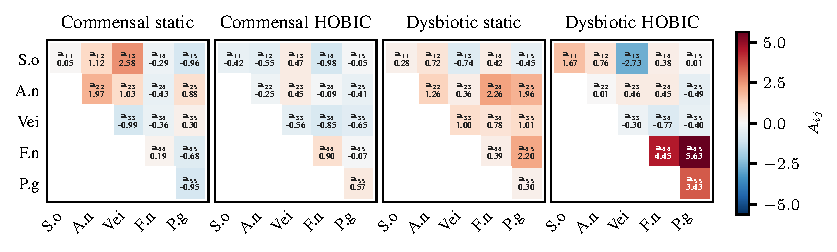
\includegraphics[width=\textwidth]{figures/heatmap_A_4cond.pdf}
\caption{MAP interaction matrices $\mathbf{A}$ (Phase~2, stage (iv)). Red: cooperative ($A_{ij}>0$); blue: competitive ($A_{ij}<0$). In commensal conditions (CS, CH), the Fn and Pg rows/columns are near zero; no entry is fixed a priori. The Fn--Pg coefficient is positive in the dysbiotic conditions.}
\label{fig:heatmaps}
\end{figure}

\subsection{Posterior parameter distributions}

Figure~\ref{fig:posterior} shows the posterior distributions of the 15 interaction matrix entries across all four conditions.
In commensal conditions (CS, CH), the Pg-related parameters ($a_{15}$, $a_{25}$, $a_{35}$, $a_{45}$, $a_{55}$) are not distinguishable from zero, although none of them is fixed a priori.
In dysbiotic conditions (DS, DH), several of these parameters shift to positive values with broader distributions \TBD{check which with final runs}.
DS exhibits the narrowest posteriors overall \TBD{check with final runs}.
% The intrinsic growth-rate parameters $\mu_i$ (not shown) are estimated jointly but exhibit negligible condition dependence, consistent with the growth rate parity reported in Section~\ref{sec:validation}.

\begin{figure}[htbp]
\centering
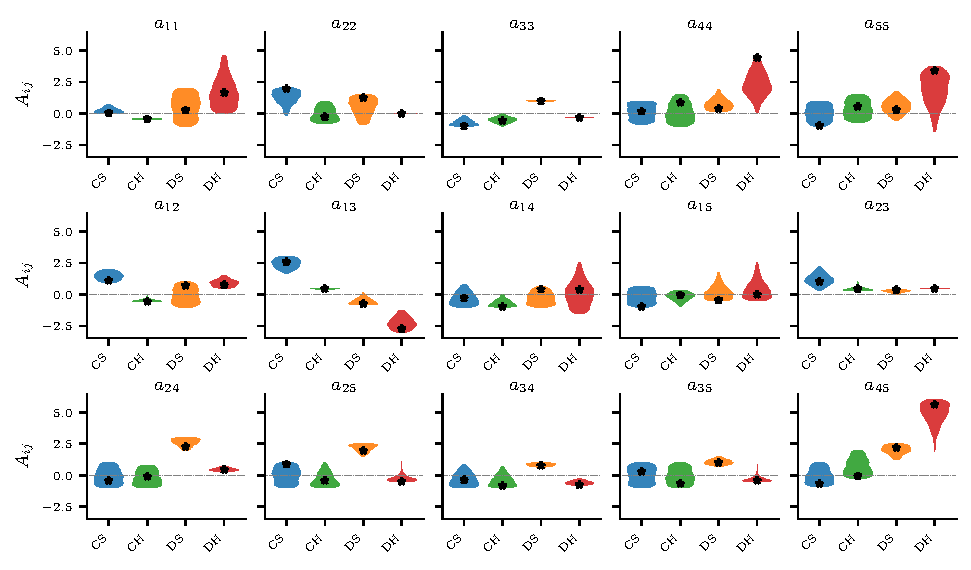
\includegraphics[width=\textwidth]{figures/paper_posterior_violin_sharey.pdf}
\caption{Posterior distributions of the 15 interaction matrix entries (Phase~2, stage (iv)). Stars: MAP estimates. Whether a narrow marginal reflects the data or the prior box is assessed in Section~\ref{sec:sensitivity}.}
\label{fig:posterior}
\end{figure}

\subsection{Quantitative comparison across conditions}
To quantify the inter-condition differences, we compute for each pair $(c_1,c_2)$ the correlation coefficient and relative Frobenius distance:
\begin{equation}
\rho^{(c_1,c_2)} = \mathrm{corr}\bigl(\mathrm{vec}(\mathbf{A}^{(c_1)}),\mathrm{vec}(\mathbf{A}^{(c_2)})\bigr),
\quad
\Delta_F^{(c_1,c_2)} = \frac{\|\mathbf{A}^{(c_1)}-\mathbf{A}^{(c_2)}\|_F}
{\max\{\|\mathbf{A}^{(c_1)}\|_F,\|\mathbf{A}^{(c_2)}\|_F\}}.
\label{eq:frob}
\end{equation}

\noindent
\begin{minipage}[c]{0.38\textwidth}
\centering\small
\begin{tabular}{@{}cc|ccc@{}}
\toprule
\textbf{C1} & \textbf{C2} & $\rho$ & $\Delta_F$ & $d_{15\mathrm{D}}$\\
\midrule
CH & CS & $+0.26$ & $1.06$ & $\mathbf{3.38}$\\
DH & DS & $\mathbf{+0.40}$ & $\mathbf{0.88}$ & $5.86$\\
CH & DH & $+0.24$ & $1.01$ & $6.33$\\
CH & DS & $-0.27$ & $1.27$ & $4.88$\\
DH & CS & $\mathbf{-0.49}$ & $1.28$ & $\mathbf{7.77}$\\
CS & DS & $-0.27$ & $\mathbf{1.36}$ & $5.88$\\
\bottomrule
\end{tabular}
\vspace{4pt}
\captionof{table}{Pairwise comparison of MAP interaction matrices. $\rho$: correlation of vectorised $\mathbf{A}$; $\Delta_F$: relative Frobenius distance; $d_{15\mathrm{D}}$: posterior centroid distance in 15D A-matrix space.}
\label{tab:pairwise}
\end{minipage}%
\hfill
\begin{minipage}[c]{0.5\textwidth}
\centering
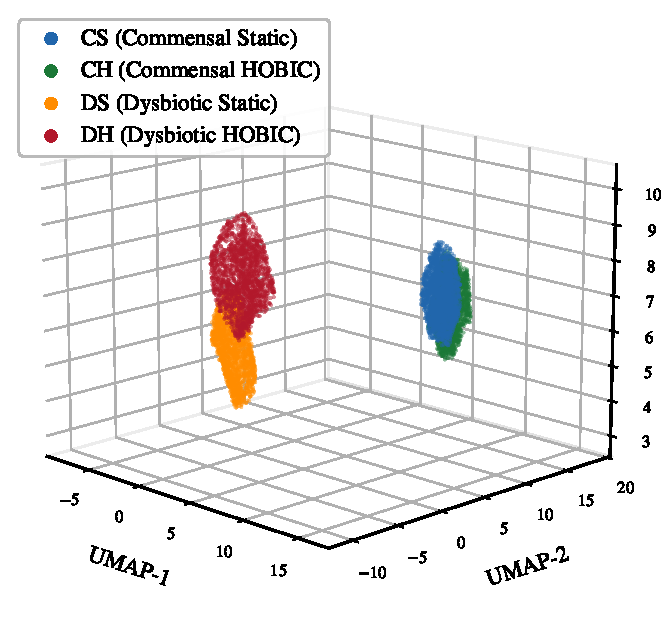
\includegraphics[width=\textwidth]{figures/umap_A_matrix_3d.pdf}
\vspace{-20pt}
\captionof{figure}{UMAP 3D embedding of posterior A-matrix samples (Phase~2, stage (iv)). The four conditions form well-separated clusters.}
\label{fig:umap}
\end{minipage}

The results (Table~\ref{tab:pairwise}) show that matrices within the same health state share a common backbone ($\rho_{\text{CH--CS}}=+0.26$, $\rho_{\text{DH--DS}}=+0.40$), whereas cross-state comparisons yield negative correlations ($\rho_{\text{DH--CS}}=-0.49$) and large Frobenius distances ($\Delta_F\geq0.88$).
The UMAP embedding of the full posterior (Figure~\ref{fig:umap}) confirms that all four conditions form well-separated clusters with no overlap~\citep{McInnes2018UMAP}; centroid distances in 15D space mirror the MAP ordering (CS--CH closest at $d\!=\!3.38$; CS--DH most distant at $d\!=\!7.77$).
Overall, the transition from health to disease corresponds to a structural reorganisation of the interaction landscape, not merely a rescaling of existing coefficients.

\subsection{Post hoc consistency checks}
\label{sec:validation}

We compare the inferred trajectories with measurements of \citet{heine2025influence} that are related to, but not identical with, the composition data.
These comparisons are consistency checks rather than independent validation.
\textit{pH} ($R^2=\TBD{0.78}$, RMSE $=\TBD{0.13}$ pH units):
the pH time series of the HOBIC conditions is not used in the inference.
A linear relation between pH and the measured species fractions is fitted once, by ordinary least squares on the experimental data alone ($N=90$ HOBIC time points, commensal and dysbiotic combined; leave-one-out RMSE $=0.056$), selecting the predictors by leave-one-out cross-validation:
\begin{equation}
  \mathrm{pH}(t) = 6.10 + 0.16\,\phi_{\mathrm{So}} + 0.55\,\phi_{\mathrm{An}} + 0.30\,\phi_{\mathrm{Vei}} + 1.22\,\phi_{\mathrm{Fn}} + 1.88\,\phi_{\mathrm{Pg}}.
  \label{eq:ph_check}
\end{equation}
Applying Eq.~\eqref{eq:ph_check} with fixed coefficients to the species fractions predicted from \TBD{500} posterior samples of stage~(iv) reproduces the measured pH of CH and DH with $R^2=\TBD{0.78}$ (\TBD{12} points).
The pH data enter only the fit of Eq.~\eqref{eq:ph_check} on measured fractions, never the inference; the check therefore tests whether the inferred model reproduces the species fractions that drive the pH, not the pH mechanism itself.

\textit{Gingipain--\textit{Pg} correlation} ($r=\TBD{0.90}$):
the temporal profile of gingipain (\citealp{heine2025influence}, Fig.~4B), the principal virulence factor of \textit{Pg}, correlates with the predicted Pg trajectory in DH, both increasing at Day~15--21; this is a temporal correlation, not a test of a mechanism.

\textit{Metabolic sign consistency}:
the MAP \textit{So}--\textit{An} coefficient ($a_{12}=\TBD{+0.76}$) is consistent with co-aggregation and cross-feeding between these early colonisers, while the \textit{So}--\textit{Vei} coefficient is negative ($a_{13}=\TBD{-2.73}$); this is a property of the effective model and should not be read as evidence against the well-established lactate cross-feeding between streptococci and \textit{Veillonella}.

% Removed pH validation (pH now enters the Phase-2 likelihood):
% \subsection{Independent validation}
% \label{sec:validation}
%
% We validate the Phase~2 MAP parameters against four measurements from \citet{heine2025influence} that were \emph{not} used in calibration.
%
% \textit{pH prediction} (LOO-$R^2 = 0.920$; independent $R^2 = 0.777$):\textit{Model selection.}
% Candidate linear regressors were evaluated by leave-one-out cross-validation (LOO-CV) on $N=90$ HOBIC time points (0.5-day resolution, commensal and dysbiotic combined).
% Four nested models were compared---So+$V_{\mathrm{ei}}$, So+Fn, So+Fn+Pg, So+An+Fn+Pg---and extended by $\phi_{\mathrm{Vei}}$ as a fifth predictor.
% The five-predictor model yielded the best independent validation performance and was selected:
% \begin{equation}
%   \mathrm{pH}(t) = 6.10 + 0.16\,\phi_{\mathrm{So}} + 0.55\,\phi_{\mathrm{An}}
%                         + 0.30\,\phi_{\mathrm{Vei}} + 1.22\,\phi_{\mathrm{Fn}} + 1.88\,\phi_{\mathrm{Pg}}
%   \label{eq:ph_regression}
% \end{equation}
% (LOO-RMSE~$= 0.056$; coefficients estimated by ordinary least squares on experimental species fractions).
% Species--pH Pearson correlations confirm the mechanistic roles: $\phi_{\mathrm{Fn}}$ ($r=+0.93$) and $\phi_{\mathrm{Pg}}$ ($r=+0.93$) are the dominant pH drivers, with alkalinisation attributable to gingipain-mediated arginine and lysine catabolism releasing ammonia; $\phi_{\mathrm{So}}$ contributes acidification ($r=-0.68$) via lactic acid production.
%
% \textit{Independence test.}
% The regression coefficients of Eq.~(\ref{eq:ph_regression}) were fixed from experimental data.
% To evaluate the predictive power of the inferred $\mathbf{A}$ matrix, we drew 500 samples from the Phase-2 TMCMC posterior ($10\,000$-particle TMCMC) and integrated the Hamilton ODE forward using Day-1 experimental species fractions as initial conditions, yielding posterior species trajectories $\phi_i(t)$ at $t=1,3,6,10,15,21$\,days.
% Applying the fixed $\beta$ coefficients to these ODE-predicted fractions---without any access to pH data during TMCMC calibration---gives $R^2 = 0.777$ (RMSE~$= 0.126$\,pH units) against the held-out HOBIC pH time series (Fig.~\ref{fig:ph_validation}), confirming that the inferred interaction matrix $\mathbf{A}$ captures the community drivers of pH.
%
% \begin{figure}[htbp]
%   \centering
%   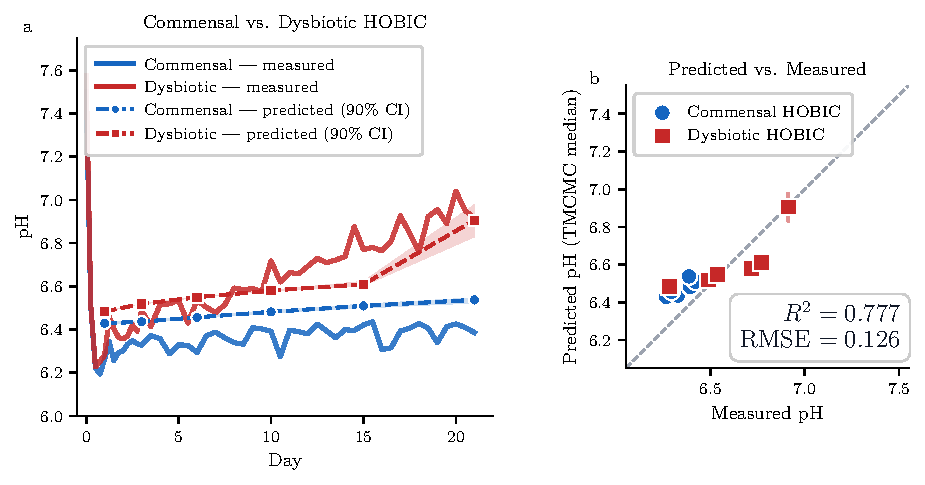
\includegraphics[width=\textwidth]{figures/fig_ph_validation.pdf}
%   \caption{Independent pH validation.
%   \textbf{(a)}~Measured HOBIC pH time series (solid lines) overlaid with TMCMC posterior predictions (dashed lines, markers) and 90\% credible intervals (shaded bands) for commensal (blue) and dysbiotic (red) conditions.
%   \textbf{(b)}~Scatter plot of TMCMC-predicted vs.\ measured pH at six time points ($t=1,3,6,10,15,21$\,days); vertical bars indicate 90\% posterior CIs.
%   Regression coefficients were fitted solely from experimental species fractions (LOO-CV, $N=90$); pH data were not used in TMCMC calibration.
%   $R^2=0.777$, RMSE~$=0.126$\,pH units ($N=12$ points, two conditions).}
%   \label{fig:ph_validation}
% \end{figure}
%
%

% \textit{Growth rate parity}:
% planktonic doubling times (1.68\,h commensal vs.\ 1.64\,h dysbiotic; Fig.~1B) confirm that condition differences arise from community interactions, not individual species fitness.

\subsection{Transferability and identifiability}
\label{sec:sensitivity}

\paragraph{Cross-condition transferability.}
To test whether the inferred matrices capture genuine condition-specific structure, we evaluate each MAP on every other condition's data (Table~\ref{tab:cross_prediction}).
Within-state commensal transfer (CS to CH) achieves an RMSE of 0.098, \emph{below} the CH self-prediction of 0.104, indicating a shared commensal interaction backbone that generalises across cultivation modes.
Cross-state transfers (DS to CS: 0.384, CS to DH: 0.198) degrade sharply, indicating that commensal and dysbiotic matrices differ.

\begin{table}[htbp]
\centering\small
\begin{tabular}{@{}lcccc@{}}
\toprule
Source $\backslash$ Target & CS & CH & DS & DH \\
\midrule
CS & \textbf{0.119} & 0.098 & 0.261 & 0.198 \\
CH & 0.257 & \textbf{0.104} & 0.100 & 0.159 \\
DS & 0.384 & 0.259 & \textbf{0.033} & 0.255 \\
DH & 0.342 & 0.212 & 0.289 & \textbf{0.087} \\
\bottomrule
\end{tabular}
\caption{Cross-condition prediction RMSE. Rows: condition whose MAP is used; columns: data. Diagonal (bold): self-prediction, equal to the calibrated RMSE.}
\label{tab:cross_prediction}
\end{table}

\paragraph{Identifiability.}
The ratio $r_i=\sigma_{\mathrm{post},i}/\Delta_{\mathrm{prior}}$ cannot detect non-identifiability: a posterior identical to a uniform prior already gives $r=1/\sqrt{12}\approx0.29$.
We therefore assess identifiability by (i)~agreement across independent seeds (Section~\ref{sec:convergence}), (ii)~the dependence of each marginal on the prior, comparing inference on the wide box $[-15,20]$ with and without an $\mathcal{N}(0,6^2)$ prior, and (iii)~the fraction of posterior mass at the box bounds.
\TBD{Result: which entries are determined by the data and which depend on the prior (DH and DS).}
Parameters whose marginals change with the prior are reported as weakly identified, and no biological interpretation is based on them.

\paragraph{Likelihood weights.}
The weights $\lambda_{\mathrm{Pg}}=5$ and $\lambda_{\mathrm{late}}=3$ (Table~\ref{tab:weights}) are modelling choices.
Repeating stage~(i) for DH with $\lambda_{\mathrm{Pg}}=\lambda_{\mathrm{late}}=1$ \TBD{result: sign and 90\% interval of $a_{45}$, Pg D21/D15 ratio and RMSE, compared with the weighted run}.

\paragraph{Necessity of the \textit{Fn}--\textit{Pg} interaction.}
We compare the full model with a reduced model in which $a_{45}=0$, both inferred from stage~(i), whose particles are initialised from the prior so that the log-evidence estimate is valid.
\TBD{Table: $\ln\hat Z$ (mean $\pm$ spread over three seeds) of both models and $\ln B=\ln\hat Z_{\mathrm{full}}-\ln\hat Z_{a_{45}=0}$ for the four conditions.}
Because the prior on $a_{45}$ is uniform, $\ln B$ includes an Occam penalty proportional to the log of the box width and is therefore conservative for the full model. The box widths differ between conditions (Supplementary Table~S1): for DS, where the box had to be widened to $[-15,20]$ (Section~\ref{sec:prior}), the penalty is $\ln 35\approx3.6$, compared with $\ln 6.5\approx1.9$ for DH. We therefore read $\ln B$ only within each condition, and compare conditions through the posterior of $a_{45}$ rather than through $\ln B$. In DS, $a_{45}$ and $a_{33}$ trade off: with $a_{45}=0$ the posterior moves almost entirely to the mode $a_{33}\approx-10$ with nearly the same fit (maximum log-likelihood \TBD{$-1.5$ versus $-0.6$}), whereas the full model places most of its mass at $a_{33}\approx+1$ with $a_{45}>0$. The relative weight of the two $a_{33}$ modes is not reliably determined by the data, and we therefore report $a_{45}$ for DS separately for each mode: in the mode $a_{33}\approx+1$, which carries most of the mass and fits better (maximum log-likelihood higher by 0.6--1.2), $a_{45}=\TBD{+2.4}$ with a 90\% interval excluding zero (\TBD{$[+0.5,+4.4]$}); in the mode $a_{33}\approx-10$, $a_{45}=\TBD{+0.8}$ with an interval that includes zero (\TBD{$[-0.2,+1.4]$}). The evidence for $a_{45}>0$ in DS is therefore conditional on the $a_{33}$ mode, unlike in DH.

%==============================================================================
\section{Discussion}
\label{sec:discussion}
%==============================================================================

\paragraph{Biological interpretation.}
The inferred interaction matrices provide a quantitative, effective description of the commensal and dysbiotic community states.
Under commensal conditions, the dominant coefficients involve the early colonisers \textit{So}, \textit{An} and \textit{Vei}, consistent with their reported co-aggregation and cross-feeding. Under dysbiotic conditions, the effective \textit{Vei}--\textit{Pg} and \textit{Fn}--\textit{Pg} coefficients become positive, with magnitudes that depend on the cultivation regime, whereas the Pg-related coefficients in both commensal conditions are not distinguishable from zero.
Differences between commensal and dysbiotic matrices combine the effect of community state with those of the \textit{Veillonella} species (\textit{V.~dispar} vs.\ \textit{V.~parvula}) and the Pg strain (DSM\,20709 vs.\ W83), and cannot be attributed to the community state alone.

Matrices within the same community state are positively correlated, whereas cross-state comparisons are \TBD{anticorrelated} (Table~\ref{tab:pairwise}).
Together with the cross-condition transfer (Table~\ref{tab:cross_prediction}), in which MAP estimates transfer within community states across cultivation modes but not across states, this indicates that the commensal and dysbiotic data require different interaction matrices rather than a rescaling of a shared one \TBD{re-check both tables with the final runs}.

\paragraph{A testable prediction.}
Beyond reproducing the observed community states, the inferred model yields a specific prediction.
In posterior predictive simulations of the dysbiotic dynamic condition, the late Pg increase (Day-21/Day-15 ratio $\ge1.5$) occurs in \TBD{99--100}\% of posterior samples.
Removing \textit{F.~nucleatum} from the consortium (its volume fraction held at zero) reduces this to \TBD{10--13}\%, and setting only the Fn--Pg coefficient $a_{45}$ to zero reduces it to \TBD{2--6}\%.
The late increase thus arises in the model from a delayed rise of \textit{F.~nucleatum} transmitted to Pg through $a_{45}$, consistent with the bridging role of \textit{F.~nucleatum}~\citep{Kolenbrander2010OralMultispecies}.
The model therefore predicts, with posterior probability \TBD{0.87--0.90}, that a leave-\textit{F.~nucleatum}-out co-culture under otherwise identical dynamic cultivation suppresses the late Pg increase.
Because commensal and dysbiotic consortia differ in \textit{Veillonella} species and Pg strain as well as in community state, the prediction concerns this consortium and should not be generalised to other strain combinations.

\paragraph{Effect of the viability and pH data.}
Figure~\ref{fig:phase_scatter} compares the Phase~1 (composition only) and Phase~2 (with viability and pH) MAP estimates parameter by parameter.
In commensal conditions, the two phases yield consistent MAPs ($r=\TBD{0.83}$--$\TBD{0.90}$): the additional data change $\mathbf{A}$ little.
In dysbiotic conditions, the MAPs differ more ($r=\TBD{0.23}$ for DS, $\TBD{0.62}$ for DH), with the largest shifts in Pg-related parameters, where the measured viability changes most.
The viability predictions themselves remain approximate (RMSE \TBD{0.11--0.39}), indicating that the $\psi$-dynamics of the model capture the loss of membrane integrity only coarsely; the viability channel acts mainly as an additional constraint on $\mathbf{A}$.

\begin{figure}[htbp]
\centering
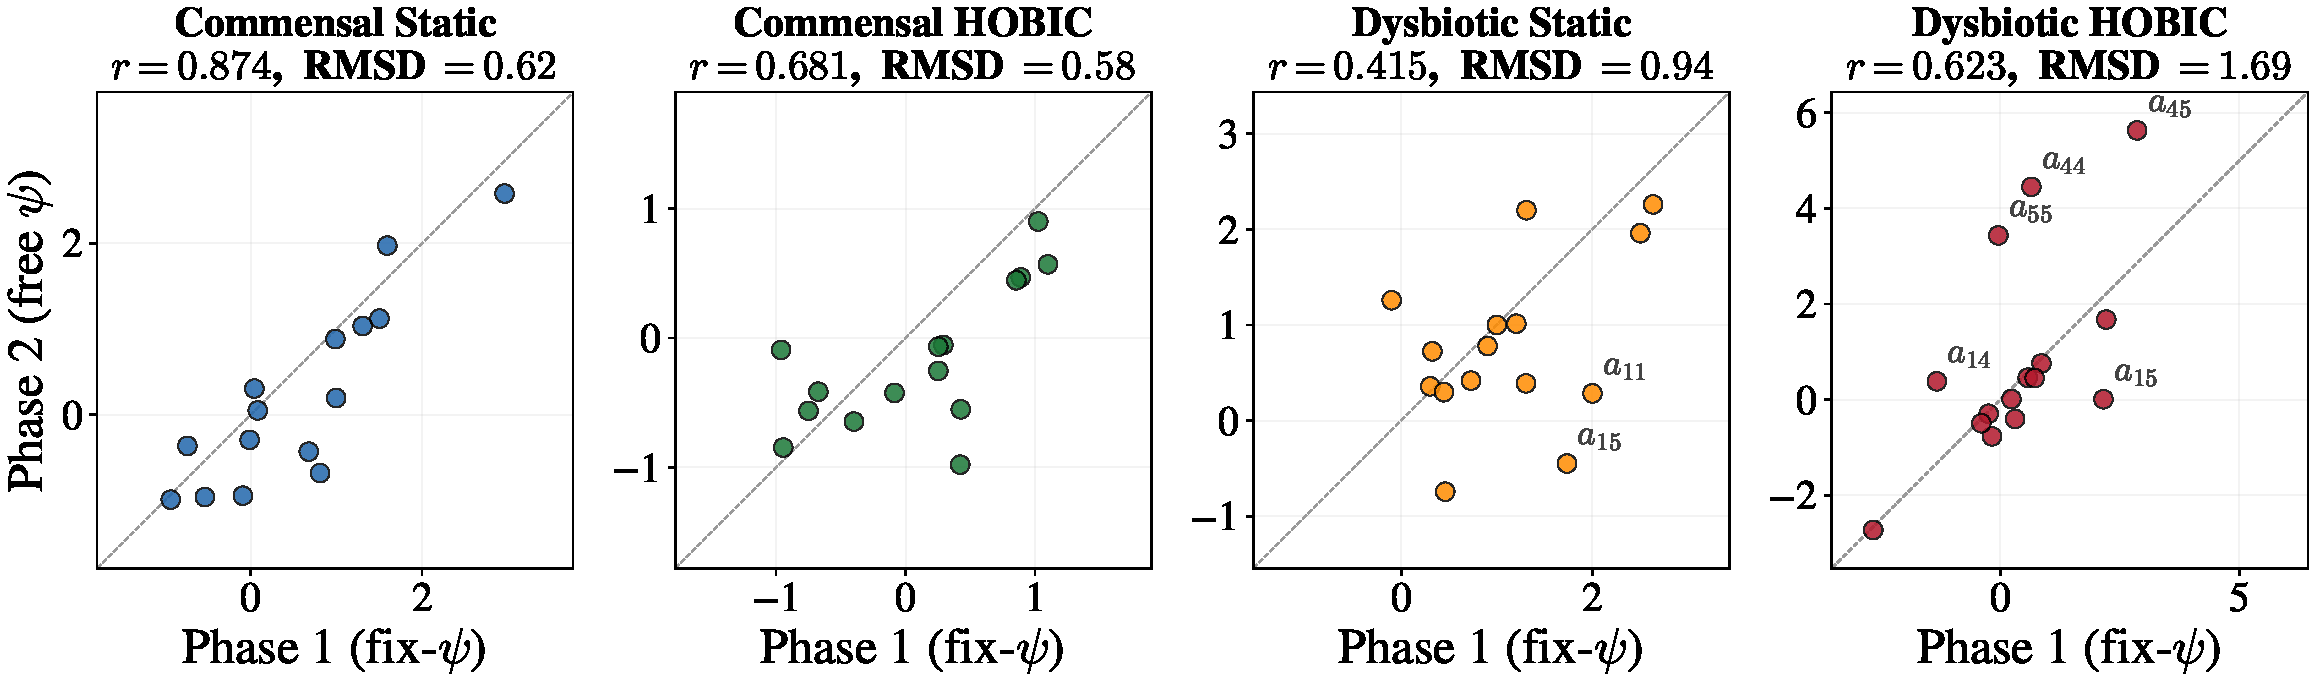
\includegraphics[width=\textwidth]{figures/phase1_vs_phase2_map.pdf}
\caption{Phase~1 (composition only) vs.\ Phase~2 (with viability and pH) MAP estimates. Each point is one of the 15 parameters; dashed line: identity. \TBD{update with the final runs}}
\label{fig:phase_scatter}
\end{figure}

\paragraph{Computational considerations.}
The $\sim$150$\times$ GPU speedup (Table~\ref{tab:timing}) exploits the embarrassingly parallel mutation step via \texttt{jax.vmap}.
For this solver and workload, gradient-based samplers (HMC, NUTS) were less efficient on the GPU, because trajectories of variable length limit batched evaluation~\citep{Dance2025FSM}.
Combining the direct-ODE approach with surrogate acceleration~\citep{Fritsch2025BayesianMicrofilms} is a natural extension.

%==============================================================================
\section{Conclusions}
\label{sec:conclusions}
%==============================================================================

We have presented a GPU-accelerated Bayesian framework for estimating the interaction parameters of a five-species oral biofilm model.
The key contributions are:

\begin{enumerate}[nosep,leftmargin=*]
\item \textbf{Staged inference with explicit convergence checks.}
The interaction matrix is first inferred from the species composition and then refined with the viability data; every stage is run with three seeds and accepted only if explicit convergence criteria hold.
All 15 parameters are estimated without fixing any of them a priori; the Pg-related coefficients in the commensal conditions are not distinguishable from zero.

\item \textbf{GPU-accelerated TMCMC.}
Compiling the forward model via JAX and batching all particles on GPU achieves a $\sim$150$\times$ speedup (Table~\ref{tab:timing}), making repeated runs with up to $N_p=5{,}000$ particles feasible.

\item \textbf{Reproduction of four conditions and a testable prediction.}
The framework reproduces commensal homeostasis (CS, CH), moderate dysbiosis (DS), and the late Pg increase (DH).
Posterior predictive simulations predict that removing \textit{F.~nucleatum} suppresses the late Pg increase under dysbiotic dynamic cultivation, which can be tested by a leave-one-species-out co-culture.

\item \textbf{Quantitative interaction comparison.}
Pairwise comparison and cross-condition transfer indicate that commensal and dysbiotic data require different interaction matrices, whereas matrices within a community state transfer across cultivation modes.

\item \textbf{Identifiability.}
Identifiability is assessed by seed agreement, prior dependence on a wide box and the posterior mass at the bounds, rather than by the posterior-to-prior width ratio, which cannot detect non-identifiability; \TBD{summary of which entries are identified}.
\end{enumerate}

\paragraph{Future work.}
\begin{itemize}[nosep,leftmargin=*]
    \item \textbf{Experimental test of the prediction:} a leave-\textit{F.~nucleatum}-out co-culture under dysbiotic dynamic cultivation.
    \item \textbf{External validation:} testing the inferred interactions against independent in-vivo datasets (e.g., \citet{dieckow2024structure}).
    \item \textbf{Spatially resolved inference:} coupling the framework to the continuum PDE biofilm model~\citep{Klempt2025ContinuumBiofilm} to exploit depth-resolved FISH/CLSM imaging.
\end{itemize}

\backmatter

\bmhead{Acknowledgements}
The authors acknowledge the Lower Saxony Centre for Biomedical Engineering, Implant Research and Development (NIFE), Hannover.
Computational resources of the Multiphysics Materials Computation Research Group (Assoc.\ Prof.\ M.~Muramatsu), Department of Mechanical Engineering, Keio University, are gratefully acknowledged.

\section*{Statements and Declarations}

\bmhead{Funding}
This work was funded by the Deutsche Forschungsgemeinschaft (DFG, German Research Foundation) under the Collaborative Research Center SFB/TRR-298-SIIRI -- Project ID 426335750.
Funded by the European Union (ERC, Gen-TSM, project number 101124463). Views and opinions expressed are however those of the author(s) only and do not necessarily reflect those of the European Union or the European Research Council Executive Agency. Neither the European Union nor the granting authority can be held responsible for them.

\bmhead{Competing interests}
The authors declare no competing interests.

\bmhead{Ethics approval and consent to participate}
Not applicable. This study analyses previously published in-vitro data and involves no human participants or animals.

\bmhead{Data availability}
This study analyses previously published data. The experimental time courses were reported by \citet{heine2025influence} and are available from that publication; they are not redistributed with this article.

\bmhead{Code availability}
Code, run configurations, convergence records and posterior samples are archived at Zenodo (\TBD{DOI}) and developed at \url{https://github.com/keisuke58/Tmcmc202601}.

\bmhead{Author contributions}
\TBD{draft, to be confirmed by all co-authors}
K.N.\ and P.J.\ conceived the study.
K.N.\ developed the inference framework, implemented the GPU/JAX forward model and the TMCMC sampler, performed the analyses, and drafted the manuscript.
F.K.\ and H.G.\ contributed the continuum biofilm model and its numerical formulation; M.So.\ contributed to the variational formulation and numerical methods.
N.H.\ designed and performed the in-vitro biofilm experiments and curated the time-course data.
K.D.-N.\ provided imaging resources and data and contributed to data interpretation.
R.M.\ and S.P.S.\ contributed experimental data and biological interpretation.
M.St.\ provided clinical context and resources.
P.J.\ supervised the study and acquired funding.
All authors critically reviewed and approved the final manuscript.

%==============================================================================
\bibliography{references_ikm}
%==============================================================================

%==============================================================================
% \newpage
% \appendix
% \section*{Supplementary Material}
% \addcontentsline{toc}{section}{Supplementary Material}
% %==============================================================================

% \subsection*{S1\quad KEGG/eHOMD metabolic sign-consistency analysis}
% \label{sec:supp_kegg}

% \paragraph{Net-flow matrix construction.}
% To assess whether the inferred interaction matrices are consistent with known metabolic biochemistry, we constructed a $5\times5$ net-flow matrix $F$ from two sources.
% First, we parsed Supplementary File~1 of \citet{Dieckow2025InVivo}, which catalogues microbe--metabolite--enzyme relationships annotated with KEGG and HMDB identifiers for the five focal genera.
% For each metabolite, a weight $w=2$ was assigned to KEGG/HMDB-confirmed interactions and $w=1$ to literature-only entries; entries in which one taxon \textsc{produces} a metabolite that another taxon \textsc{uses} incremented $F_{\mathrm{tgt,src}}$ by $w$, while \textsc{inhibits} relationships decremented it.
% Second, four mutualistic pairs absent from the Dieckow supplement but supported by eHOMD and primary literature (So--An lactate cross-feeding; An--Fn bridge synergy; Vd--Fn metabolite exchange; Fn--Pg coaggregation) were added with weight $w=1$.
% The resulting signed matrix $F = F^+ - F^-$ has 16 non-zero off-diagonal entries and is common to all four conditions.

% \paragraph{Soft sign prior.}
% During TMCMC estimation, a half-normal penalty was appended to the log-posterior for each non-zero entry of~$F$:
% \begin{equation}
%   \log p_{\mathrm{sign}}(\mathbf{A}) =
%   -\sum_{i \neq j,\, F_{ij}\neq 0}
%   \frac{|F_{ij}|}{2\sigma_{\mathrm{KEGG}}^2}
%   \bigl[\max(0,\,-\operatorname{sgn}(F_{ij})\,A_{ij})\bigr]^2,
%   \label{eq:sign_prior}
% \end{equation}
% with $\sigma_{\mathrm{KEGG}}=0.15$ for CS, CH, and DH, and $\sigma_{\mathrm{KEGG}}=0.08$ for DS.
% The penalty is zero when $A_{ij}$ has the correct sign or is negligibly small, and grows quadratically for wrong-sign entries proportional to the KEGG/HMDB evidence weight.
% The tighter $\sigma$ for DS was selected by cross-validating on sign agreement: strengthening the prior from 0.15 to 0.08 raised SA from 62\,\% to 75\,\% with a negligible change in MAP log-likelihood ($\Delta\log L = -0.026$), while the same tightening for DH degraded the MAP log-likelihood by 39 units without improving SA, confirming that the DH discordances are data-driven rather than sampling artefacts.

% \paragraph{Sign-agreement results.}
% Sign agreement (SA) is evaluated on the posterior mean $\bar{\mathbf{A}}$ (average over all TMCMC samples) against the 16 non-zero off-diagonal pairs of $F$, using a threshold $|A_{ij}|>0.02$ to exclude negligible entries.
% Figure~\ref{fig:kegg_sign} shows the posterior mean $\bar{\mathbf{A}}$ (top row) and the MAP $\hat{\mathbf{A}}$ (bottom row) for each condition; lime borders indicate sign agreement with $F$, red borders disagreement.

% \begin{itemize}[nosep,leftmargin=*]
%   \item \textbf{CS and CH (commensal):} 16/16 pairs (100\%) agree with KEGG/eHOMD predictions, confirming that metabolite-mediated mutualism is the dominant organising principle in healthy biofilms.
%   \item \textbf{DS (dysbiotic static):} 12/16 pairs (75\%) agree.
%         The four discordant pairs involve \textit{F.~nucleatum} interactions (Fn--So, Fn--Vd), where the posterior assigns negative coefficients despite KEGG-predicted cross-feeding, and the Pg--So pair.
%   \item \textbf{DH (dysbiotic HOBIC):} 12/16 pairs (75\%) agree.
%         The primary discordance is $A_{\mathrm{Fn,So}}=-0.73$, indicating that under dysbiotic flow conditions \textit{F.~nucleatum} and \textit{S.~oralis} compete rather than cooperate---consistent with spatial exclusion in a shear-driven environment.
% \end{itemize}

% The residual discordances in dysbiotic conditions reflect genuine data-driven ecological dynamics---competitive exclusion overriding metabolite-mediated mutualism---rather than inference artefacts.
% This pattern is ecologically coherent: dysbiotic conditions enrich virulence-associated strains (Pg W83) that may alter the redox and substrate environment in ways not captured by the KEGG metabolic network alone.

% \begin{figure}[htbp]
%   \centering
%   \includegraphics[width=\textwidth]{figures/fig_heine_kegg_sign_comparison.png}
%   \caption{%
%     \textbf{KEGG/eHOMD sign-consistency of the inferred Hamilton TMCMC interaction matrices.}
%     \textit{Top row:} posterior mean $\bar{\mathbf{A}}$;
%     \textit{Bottom row:} MAP estimate $\hat{\mathbf{A}}$.
%     Cell colour encodes interaction strength (red\,=\,negative, blue\,=\,positive);
%     lime (red) borders indicate sign agreement (disagreement) with the net-flow matrix~$F$.
%     Commensal conditions achieve 100\,\% sign agreement in both statistics;
%     dysbiotic conditions reach 75\,\%, with discordant Fn interactions reflecting
%     competitive exclusion dynamics absent from the KEGG metabolite network.
%   }
%   \label{fig:kegg_sign}
% \end{figure}

\end{document}
